\documentclass[10pt]{article}

\usepackage[dvips]{graphicx}
\graphicspath{{./eps/}}
\DeclareGraphicsExtensions{.eps}

\usepackage{amsmath}
\usepackage{verbatim}
\usepackage{color}

\begin{document}

\author{Freddy Chua}
\title{Event/Anomaly/Fault Detection}

\maketitle

\section{Model}

For the road connecting two bus stops, we call it a segment. We assume that every segment has a speed associated with it. A bus traveling from a point of origin $x$ to its destination $y$ goes through a sequence of segments. Instead of assuming a constant speed associated with the route, we assume that the route can be divided into multiple segments, where each segment takes on a speed of its own. Given that a journey $n$ starts at $x$ and ends at $y$, a route taken by $n$ is denoted by $r_n(x_n, y_n)$ ($r_n$ for brevity).
%An edge that belongs to $r_n(x_n, y_n)$ connects two other nodes which could intersect with the route of others.

%Suppose there are $N$ journeys, $r_n(x_n, y_n)$ denotes one of the journey $n$. 
Given that $i$ is the starting point and $j$ is the ending point within each segment $(i, j)$, let $d_{i,j}$ be the distance associated with this segment and $c_{i,j}$ be the speed associated with this segment.

The predicted time $\hat{t}_n$ of the journey is given by the following Gaussian distribution,
\begin{gather}
\hat{t}_n \sim \mathcal{N} \left( \sum_{ (i,j) \in r_n } \frac{ d_{i,j} }{ c_{i,j} }, d_{x_n, y_n} \sigma^2 \right)
\end{gather}

\begin{comment}
	\subsection{Estimation of the Mean using Least Squares Error}

	To estimate the speed $c_{i,j}$ of every segment $(i,j)$ using the observed time of the journey $t_n$, we formulate the following objective function based on minimizing the least squares error\footnote{Maximizing the Log Likelihood would give similar results} between the observed time $t_n$ and predicted time $\hat{t}_n$,

	\begin{align*}
	\mathcal{L} &= \sum_{n} \left( t_n - \hat{t}_n \right)^2 - \tau \sum_{(i,j) \in E} \log(c_{i,j}) \\
	&= \sum_{n} \left( t_n - \sum_{ (i,j) \in r_n(x_n, y_n) } \frac{d_{i,j}}{c_{i,j}} \right)^2 - \tau \sum_{(i,j) \in E} \log(c_{i,j}) \\
	\frac{d \mathcal{L}}{d c_{i,j}} &= \sum_{n} 2 \left( t_n - \sum_{ (i,j) \in r_n(x_n, y_n) } \frac{d_{i,j}}{c_{i,j}} \right) \frac{d_{i,j}}{c_{i,j}^2} - \frac{\tau}{c_{i,j}}
	\end{align*}

	Using Stochastic Gradient Descent, we would be able to update $c_{i,j}$ using each trip information $n$ as follows,
	\begin{gather}
	c_{i,j}^{new} = c_{i, j}^{old} - \eta \left[ \left( t_n - \sum_{ (i,j) \in r_n(x_n, y_n) } \frac{d_{i,j}}{c_{i,j}} \right) \frac{d_{i,j}}{c_{i,j}^2} - \frac{\tau}{c_{i,j}} \right]
	\end{gather}
\end{comment}

\subsection{Estimation of the Mean by Maximum Log Likelihood}

The log likelihood as contributed by each trip $n$ is given by, 
\begin{align}
	\mathcal{L} &= \log \left( \frac{1}{\sqrt{2 \pi d_{x_n, y_n} \sigma^2 }} \right) - \frac{\left( t_n - \sum_{ (i,j) \in r_n } \frac{d_{i,j}}{c_{i,j}} \right)^2}{2 d_{x_n, y_n} \sigma^2 } \nonumber \\
	&= - \frac{1}{2} \log \left( d_{x_n, y_n} \sigma^2 \right) - \frac{\left( t_n - \sum_{ (i,j) \in r_n } \frac{d_{i,j}}{c_{i,j}} \right)^2}{2 d_{x_n, y_n} \sigma^2 }
\end{align}
We add a log barrier penalty to prevent negative speeds, 
\begin{align}
	\mathcal{L^*} = - \frac{1}{2} \log \left( d_{x_n, y_n} \sigma^2 \right) - \frac{\left( t_n - \sum_{ (i,j) \in r_n } \frac{d_{i,j}}{c_{i,j}} \right)^2}{2 d_{x_n, y_n} \sigma^2 } + \tau \sum_{(i,j) \in E} \log c_{i,j}
\end{align}
By taking partial derivative with respect to $c_{p,q}$,
\begin{align}
	\label{eqn:sgd_mean}
	\frac{\partial \mathcal{L}}{\partial c_{p,q}} = - \frac{\left( t_n - \sum_{ (i,j) \in r_n } \frac{d_{i,j}}{c_{i,j}} \right)}{d_{x_n, y_n} \sigma^2 } \cdot \frac{d_{p,q}}{c_{p,q}^2} + \frac{\tau}{c_{p,q}}
\end{align}
The partial derivative allows us to perform Stochastic Gradient Descent on parameters $c_{p,q}$ as follows.
\begin{align}
	c_{p,q} \leftarrow c_{p,q} + \eta \frac{\partial \mathcal{L}}{\partial c_{p,q}}
\end{align}
There are several interesting properties with the partial derivative in Equation \ref{eqn:sgd_mean}. The denominator of the variance shows that the more uncertain we are, the lesser the gradient is, hence less changes to $c_{i,j}$. The smaller $c_{i,j}$ is, the second component in Equation \ref{eqn:sgd_mean} will compensate by adding positive speed to prevent negative speeds.

\subsection{Estimation of the Variance}

To estimate the variance $\sigma^2$ in every segment $(i,j)$, 
\begin{align}
	\frac{\partial \mathcal{L}}{\partial \sigma^2} &= - \frac{1}{ 2 \sigma^2 } + \frac{ \left( t_n - \sum_{ (i,j) \in r_n } \frac{d_{i,j}}{c_{i,j}} \right)^2}{ 2 d_{x_n, y_n} \sigma^4 }
\end{align}
Solving for $\sigma^2$
\begin{align}
	\sigma^2 = \frac{ \sum_n \left( t_n - \sum_{ (i,j) \in r_n } \frac{d_{i,j}}{c_{i,j}} \right)^2}{\sum_n d_{x_n, y_n}}
\end{align}
%Then using Stochastic Gradient Descent, 
%\begin{align}
%	\sigma^2 \leftarrow \sigma^2 + \eta \frac{\partial \mathcal{L}}{\partial \sigma^2}
%\end{align}

\section{Introduction}

We perform our analysis on a transportation data set from an urbanized city, where majority of the population uses the public transportation system (PTS) which includes a network of railways and buses. 

Our main objective is to detect occurence of anomalies in the PTS in space and time. From an analytical point of view, detection of anomalies is relatively straight forward as it only requires comparision of travel times. A trip undertaken by a passenger is deemed to be anomalous if the time taken is significantly different from the average case. What is less obvious from the data set is the location of where the anomaly occured.

A basic method to detect the anomalous location is to divide the entire trip undertaken by a passenger into $N$ segments and sequentially test whether each segment is anomalous. In the worst case, such procedure would take $N$ number of tests if the last (first) segment is anomalous and the sequential test begins at the first (last) segment. A better way of testing would be to take a partitioning approach that is similar to binary search, which results in $\log N$ number of tests in the worst case. A possible way of improving beyond $\log N$ number of tests is to predict where the anomaly would most likely occur and partition the tests according to their order of probability.

Beyond the detection and localization of traffic anomalies, a more challenging task would be to understand the diffusion of anomalies within the transportation network. While several prior research has sought to understand the cause of anomalies \cite{Chawla2012,Liu2011}, we perform a more extensive study of understanding how traffic anomalies propagate throughout the transportation network, including prediction of when and where would the anomaly end, resulting in the return of smooth traffic flow to the transportation network. %(A diffusion decay model could be used here.)

%\subsection{Task}

%The immediate task is to first reconstruct the full travel details of each bus carrying the passengers. The data set does not reveal the vehicle identification plate number but only provide the service number, location and time when the passenger board or alight. Although this problem can be overcome by having the bus operators record more information such as the GPS trajectory and vehicle plate number, we currently do not have access to this information. The purpose of addressing this issue is to have an inferred temporal information of when the bus arrive and depart from the bus-stop. Once we have such information, we would be able to determine whether each segment (between two bus-stops) of the route is anomalous by comparing against the average.

%Another immediate task is to infer the route of the entire bus trip for each bus service. I think this should be done first.

\section{Data Set}

\subsection{Basic Processing}

Figure \ref{fig:trip_example} shows an example of what the data set looks like. We have the time and location of the passenger boarding and alighting from the bus for each of their travel trips. The nodes in Figure \ref{fig:trip_example} represent the bus stops while the number in the connecting edges represent the distance between two bus stops. By using the trips of various passengers in the data set, we are able to construct the route that the bus service takes, as shown in Figure \ref{fig:trip_example}. For example, from Figure \ref{fig:trip_example}, we can infer that $b$ should be between $a$ and $c$ because $b$ is nearer to $c$ compared to $a$, and $c$ is nearer to $b$ than $d$ so $d$ should come after $c$.

\begin{figure}[htb]
	\centering
	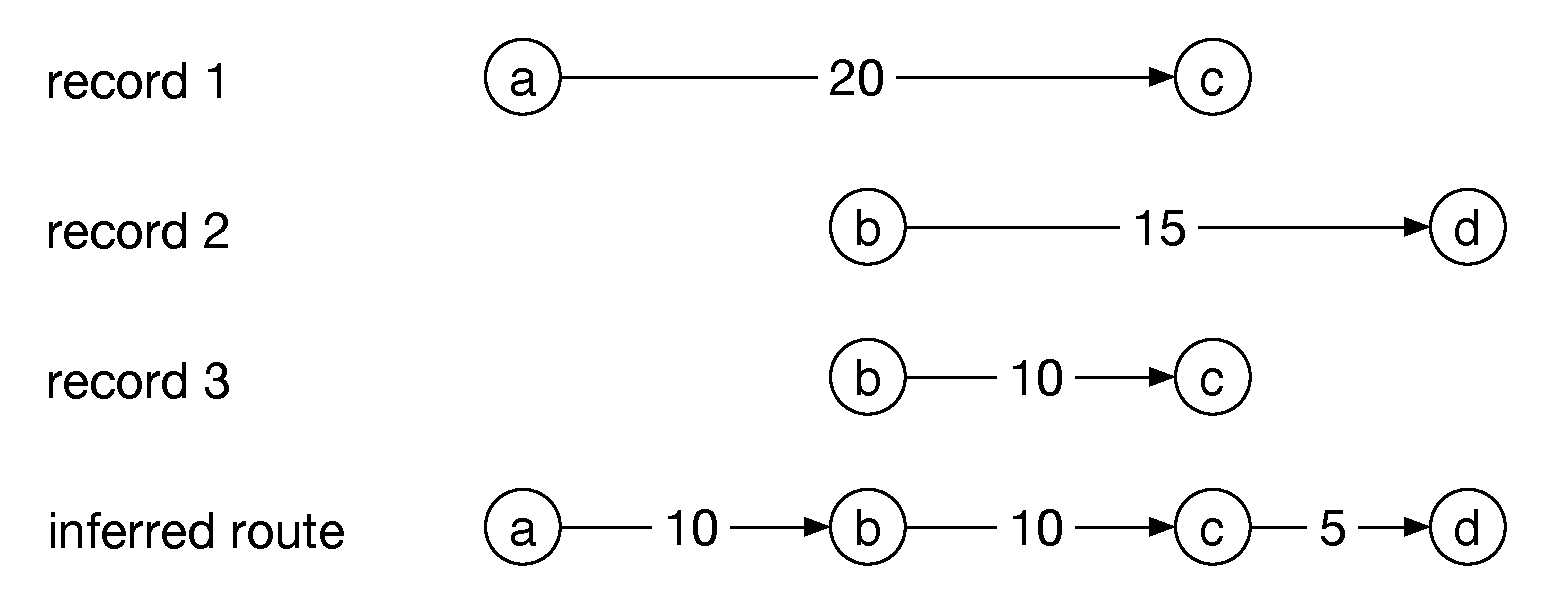
\includegraphics[width=4.0in]{trip_example}
	\caption{Examples of the trip records in the data set for a specific bus service}
	\label{fig:trip_example}
\end{figure}

Then by combining the inferred routes of various bus services, we would be able to obtain a traffic graph as shown in Figure \ref{fig:travel_graph}. Using the time information in the data set, we would be able to obtain the edges in red, which represent the roads that contain anomalies, resulting in the unpredictable timings of bus arrivals at bus stops. Because of the time information in the data set, we would have a continuous snapshot of the traffic graph at different times.

\begin{figure}[htb]
	\centering
	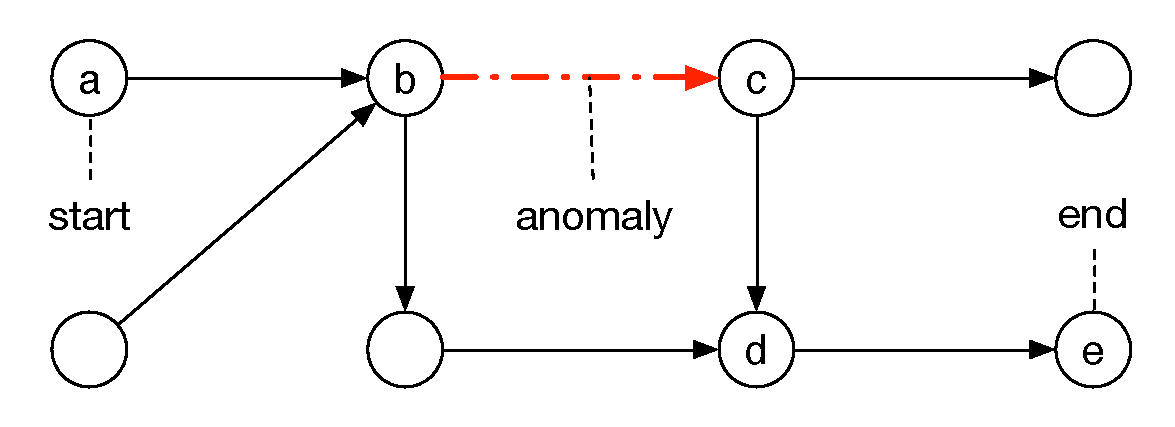
\includegraphics[width=4.0in]{travel_graph}
	\caption{Examples of the trip records in the data set for a specific bus service}
	\label{fig:travel_graph}
\end{figure}

\subsection{Empirical Observations}

\begin{figure}[htb]
	\centering
	\includegraphics[width=4.0in]{clementi_7_boarding}
	\caption{Histogram of Passengers Boarding at the First Bus Terminal}
	\label{fig:travel_graph}
\end{figure}

\begin{figure}[htb]
	\centering
	\includegraphics[width=4.0in]{bedok_7_alighting}
	\caption{Histogram of Passengers Alighting at the Last Bus Terminal}
	\label{fig:travel_graph}
\end{figure}

\section{Research Problems}

I would suggest the following few directions to take. The area of research could take us a few research papers to fully address them depending on their difficulty.

%It would only be clearer when I start working on them.

\begin{enumerate}
	\item Detecting the anomaly. Unlike other data sets such as virus propagation or spread of diseases, the anomaly in traffic data is not absolute, that is, we could only conclude with a certain degree of confidence whether there is an anomaly. What is necessary here for the traffic data set, are models that would predict the timing of bus arrival at bus stops. We would need several models here, a baseline model that ignores peak hours (the mornings' and evenings' rush hours), a model that includes off-peak and peak traveling hours, as well as models that factor in the fine grain trajectory of the bus services. Any bus arrival that falls out of the predicted schedule using the more sophisticated model would be flagged as an anomaly. I would be addressing this problem first before anything else.

	\item Finding the root cause of anomalies. This is where the problem gets more challenging from both engineering and analytical viewpoints. From the engineering perspective, it would be relatively easy to know which trip is an anomaly but difficult to pinpoint which segment of the entire trip contains the anomaly. Recall that each trip goes through a sequence of bus stops and we would like to know which road between two bus stops is an anomaly which causes the entire trip to arrive later than predicted. I would use Figure \ref{fig:group_testing_example} to illustrate how group testing might be applicable. %This is also where group testing is more likely to be applicable.

	\item Suppose we observe two anomalies happening at the same time on seemingly independent bus routes, how do we prove that these two anomalies are related, or one is the cause of the other. I would propose that we have to use quasi-experiments to separate correlation from causality. Quasi-experiments are methods in which we simulate control experiments using the data sets only, without additional real life experiments. 

	%I am still new to this, I have read about it several years back but have not done much about it.

	\item Another aspect of research is to see how traffic anomalies diffuse throughout the network. But there are already alot of work on this, and we would need to find whether traffic anomalies has any additional properties.
\end{enumerate}

\section{Regarding the Necessary Conditions of using Group Testing}

%I earlier mentioned the following two conditions in the email, let me elaborate point 1 in more detail using Figure \ref{fig:group_testing_example}.

\begin{enumerate}
\item The data set to be partitioned into groups, ideally should be non-sequential or unordered, so that the subset of the data has the flexibility of belonging to any group for testing. In this case, the transportation data set involves time, so that makes it inherently sequential and ordered. Group testing can still be used but the way of grouping the segments is restricted according to their sequence.

For example by using Figure \ref{fig:group_testing_example}, suppose we have determined that the trip from $a$ to $g$ contains an anomaly. From the data set, we do not have direct information of where the anomaly occurred. We would need to detect that the anomaly exists at the edge connecting $b$ and $c$. We could narrow the search by sequentially testing the segments $\{a, e\}, \{a, d\}, \{a, c\}, \{b, d\}$ and $\{b, c\}$. But we would not be able to group the disconnected segments $\{a, b\}$ and $\{c, d\}$ into a single test.

\begin{figure}[htb]
	\centering
	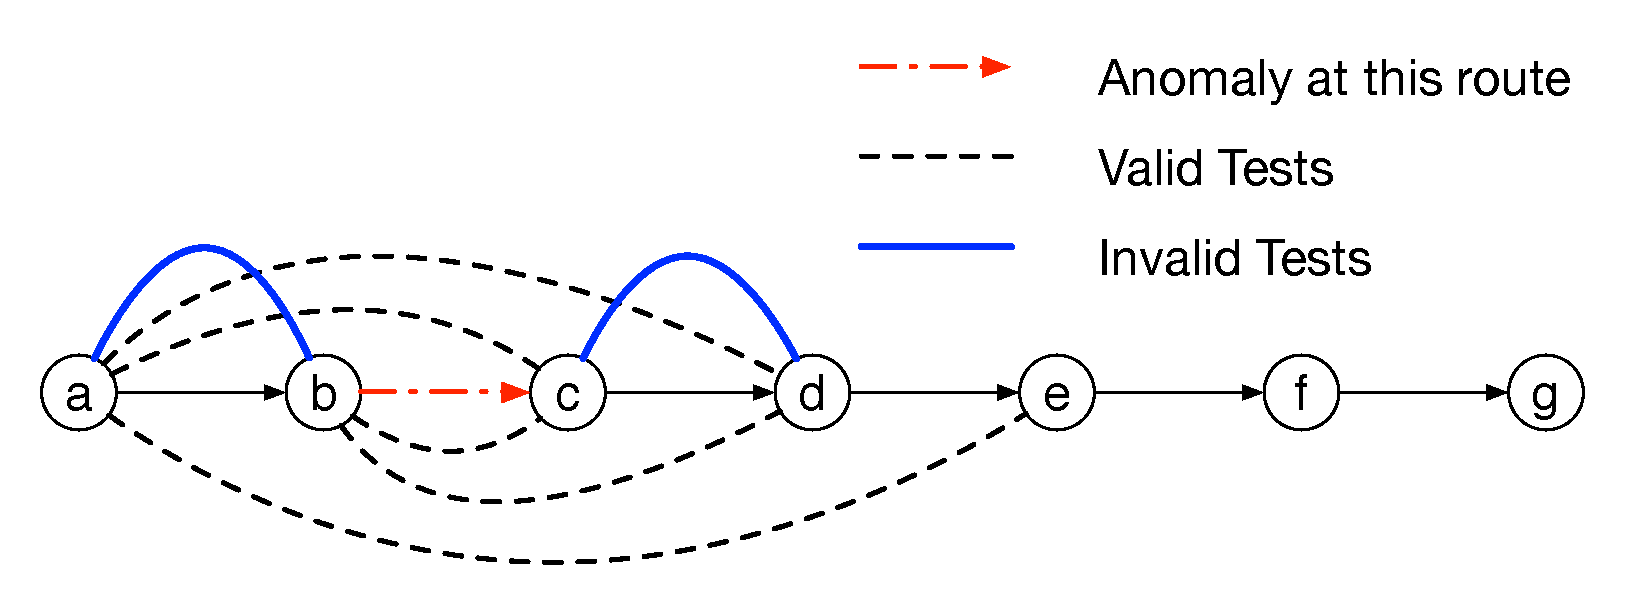
\includegraphics[width=4.0in]{group_testing_example}
	\caption{Example of Finding the Segment with Anomaly}
	\label{fig:group_testing_example}
\end{figure}

\item The test applied to the group which contains subset of the data must not change significantly when we increase the size of the group. Otherwise, it would be easier to test for each sample individually instead of aggregating them in a group.
\end{enumerate}

\section{Literature Review}

\subsection{Group Testing}

R. Dorfman proposed the use of \emph{Group Testing} to test for the presence of Syphilis \cite{Dorfman1943} among the population. The basic test requires a blood sample from each individual, which is then subjected to laboratory analysis to reveal the presence of infection. In the simplest case, a test is done for every person's sample to reveal signs of infection. 

Due to the high cost of testing, there is a necessity to reduce the number of tests required in order to weed out the infected from a large pool of individuals. The solution to minimizing the number of tests is to pool the blood samples from a set of individuals and testing the aggregated mixture once for signs of infection. If no infection is found, then the members of this pool are freed from further testing, otherwise, an additional round of testing is required for each individual blood sample.

Clearly, in this two-step process, significant savings is possible only if the probability of infection $p$ is low among a population of size $N$. The probability that a group of size $M$ has to be re-tested is given by,
\[ \left[ 1 - (1-p)^M \right] \]
The number of groups after dividing into size of $M$ is given by $\frac{N}{M}$. Then the expected number of groups $E(G)$ that has to be retested is given by,
\[ E(G) = \frac{N}{M} \left[ 1 - (1-p)^M \right] \]
The expected number of tests $E(T)$ required for the two stage process can be expressed using the following calculations,
\begin{align*}
	E(T) &= \frac{N}{M} + M \cdot E(G) \\
	& = \frac{N}{M} + M \cdot \frac{N}{M} \left[ 1 - (1-p)^M \right] \\
	& = \frac{N}{M} + N \left[ 1 - (1-p)^M \right]
\end{align*}
By varying the size of the groups $M$, we would be able to control the expected number of tests $E(T)$ required. If the objective is to minimize $E(T)$, we would determine $M$ in this manner,
\begin{align*}
	\frac{d E(T)}{d M} &= - \frac{N}{M^2} + N \left[ - (1-p)^M \log(1-p) \right] \\
	\frac{N}{M^2} &= - N \left[ (1-p)^M \log(1-p) \right] \\
	\frac{1}{M^2} &= -(1-p)^M \log(1-p)
	%\log \frac{1}{M^2} &= \log \left[ - (1-p)^M \log(1-p) \right] \\
	%-2 \log M &= M \log (p-1) + \log \left[ \log(1-p) \right]
\end{align*}
The above equation has no closed form solution, but through some approximations, $M$ can then be expressed solely in terms of $p$, and we would be able to estimate the minimum expected number of tests.
%The expected minimum number of tests required would then solely depend on $p$, which 
But the value of $p$ is unknown in most cases. Prior knowledge or additional research would be able to determine the value of $p$, which will then allow us to achieve the objective of minimizing the number of tests. In the literature as elaborated by \cite{Dorfman1943,Mezard2008,Mezard2011}, a simplifying assumption is that $p$ is similar and constant for every individual in the population. 

Li et al. \cite{Li2014} has proposed a theoretical analysis of the situation where prior information on the probability of defect $p_n$ is assumed to be known.

We could propose the use of Machine Learning to estimate $p_n$ for every individual $n$ in the population, and group them accordingly. Through additional theoretical or empirical analysis, we should then prove that knowing $p_n$ lowers the number of tests required for detecting the infected as compared to knowing only $p$.

The above analysis is only for two rounds, and additional rounds of tests can be designed to further minimize the number of tests. How many rounds or how each round of tests is designed depends on the kind of group testing. There are two kinds of group testing, adaptive and non-adaptive. In adaptive group testing, the subjects to be tested in each round depends on the outcome of the test results from previous rounds. While non-adaptive group testing would have the tests arranged prior to observing any test outcomes. The procedure introduced by Dorfman \cite{Dorfman1943} represents a form of adaptive testing. The choice of group testing depends on the nature of the problem, by considering whether it is easy to perform repeated tests on limited samples.

There is an important property that is necessary for Group Testing to be relevant, i.e. The cost of the test must increase at a rate lower than the increase in size of a group. For example, the cost for testing a group size of two, must be lower than two independent tests. The rate of increase in testing costs has not been fully explored in most literature.

M\'{e}zard et al. \cite{Mezard2008} mentioned that detecting failures in distributed systems \cite{Zheng2004,Zheng2005} can be an application of Group Testing. Zheng et al. \cite{Zheng2004,Zheng2005} proposed that a set of tests should be selected to minimize the uncertainty about the state of the distributed system. A natural measurement of uncertainty is to use conditional entropy, i.e. the entropy of the distributed system conditioned on the outcome of the tests. Zheng et al. \cite{Zheng2004,Zheng2005} model a distributed system using Bayesian network and proposed an algorithm for estimating conditional entropy on the Bayesian network. The distributed system used for their experiments is synthetically generated by the INET generator \cite{Winick2002}. By using the proposed conditional entropy estimation, Zheng et al. \cite{Zheng2004,Zheng2005} were able to select the minimal set of tests to minimize the uncertainty, thus minimizing the costs of testing.

\subsection{Traffic Anomalies Detection}

Pan et al. \cite{Pan2013} address the problem of detecting and describing traffic anomalies using crowd sensing with Beijing's taxis' GPS data and China's ``Weibo''\footnote{This service resembles Twitter but is catered for the Chinese population in Chinese language.} social media data. The anomaly which Pan et al. \cite{Pan2013} identifies is the deviance in traffic volume on segments of road during some special events. The detection of anomaly is relatively direct and the focus is on increasing the efficiency of the algorithm based on two special indexing structure for the detection algorithm.

Liu et al. \cite{Liu2011} proposed the discovery of causal interactions among traffic outliers. The framework as proposed in Liu et al.\cite{Liu2011} first partitions the geographical space into regions represented by nodes in a region graph. Edges between nodes represent the traffic flow between regions. Each edge in the region graph is differentiated within each time frame. By comparing the features of each edge across different time frames, Liu et al. is able to identify the outlier travel trajectories. From the detected outliers, an outlier tree is constructed with certain rules. In the outlier tree, each node represents an outlier trajectory. The parent of an outlier node occurs before in time and the destination of the parent is the origin of the child. The cause of the outlier, is the parent.

%However to the best of our knowledge, the discovery of relationships, especially causal interactions, among detected traffic outliers has not been investigated before. In this paper we propose algorithms which construct outlier causality trees based on temporal and spatial properties of detected outliers. Frequent substructures of these causality trees reveal not only recurring interactions among spatio-temporal outliers, but potential flaws in the design of existing traffic networks. 

\cite{Ge2011,Zhang2011,Zhang2012} analyzed taxi GPS data to detect drivers who overcharge their passengers by deliberately taking the longer route to reach the destination. The general idea for finding these anomalous routes is to compare the route taken for each pickup and destination points and obtain a measure of how much it deviates from the usual routes.

Chawla et al. \cite{Chawla2012} proposed an algorithm to detect anomalies based Pinciple Component Analysis (PCA). Chawla et al. \cite{Chawla2012} represent the traffic data into two matrices, 1) the link-path matrix and the 2) link-time matrix. Then using PCA, Chawla et al. \cite{Chawla2012} is able to factorize the matrices into eigenvectors with its respective eigenvalues. The eigenvectors corresponding to large eigenvalues represent the norm, while those eigenvectors corresponding to lower eigenvalues represent the anomalies. Using these anomalies, Chawla et al. \cite{Chawla2012} tested their method to see if they could determine the root cause on synthetically generated data sets.

\begin{comment}

\section{Data Set}

The data set of interest are records of the public transportation system (PTS) in the urbanized city of Singapore. The PTS consists of the railway system and the public buses, operated by two public listed corporations. The PTS data set is provided by a government agency that exists for the purpose of ensuring that the PTS fulfill the operational needs of the city.

Each passenger in Singapore carries a payment card containing a RFID\footnote{The RFID chip allows the companies to identify the passenger and charge the fare towards their account.} chip, which functions as a method of payment for using the PTS. The passengers boarding and alighting geo-locations are recorded for each travel trip in order to charge the appropriate amount based on the distance traveled.

Singapore being one of the most densely populated city in the world, have majority of her population commuting via the PTS, as opposed to driving in privately owned vehicles. The data set thus represent an almost complete travel information of the population which would allow us to utilize it for finding useful knowledge or detecting travel-related events.

\subsection{First Degree Information}
This section contains the information that can be obtained immediately from the records in the data set. Each transaction record contains the following:

\begin{enumerate}
	\item The encrypted ID of the passenger's payment card.
	\item The time, date and location of passenger boarding onto the vehicle.
	\item The time, date and location of passenger alighting from the vehicle.
	\item The distance traveled by passenger.
	\item The type of vehicle (bus or train).
	\item If the type of vehicle is bus, the record also contains the bus service number. The bus service number would determine the fixed route that the drivers travel, and the bus stops it would stop at to pickup or alight passengers. Each bus service is served by multiple buses, each arriving at the bus stops with regular intervals. However, the data does not contain the plate number identifying which bus the passengers travel on.
\end{enumerate}

\subsection{Second Degree Information}
Each transaction record on its own does not reveal any meaningful information but combining multiple records of the same passenger or same bus service would reveal other information. We call these the second degree information. Simple processing on the first degree information would allow us to obtain the second degree information. These information once inferred, could be assumed to be correct without any form of evaluation. In this paper, we only focus on the bus records. 

\begin{enumerate}
	\item The geographical map of where the bus stops are placed in the city.
	\item The travel route of each bus service.
	\item The bus services available at each bus stop.
	\item The bus arrival times at every bus stop for each bus service.
	\item The average speed of the buses, specific for each bus service, and localized to different segments of the bus routes.
	\item The traffic conditions of Singapore's roads at different times of each day.
	\item Average distance traveled by the passengers.
	\item By using the combination of bus and railway information, we can infer the home location of each passenger, and the location of where the passenger works at. We should not try to evaluate whether this information is correct since we cannot do actual verification.
\end{enumerate}

\section{Problem Definition}

The problem which we try to address, is the inference of knowledge from the PTS data set that does not fall into the category of first and second degree information. While we have the spatial and temporal information for the origin and destination of a trip, we do not have any detail of what happens in between the two points. It is an easy task to determine whether the trip is anomalous, but difficult to infer which segment of the trip is anomalous given the current set of data.

This is where I think Group Testing is relevant for finding the specific segment that results in the trip being anomalous. 

\section{Problem Definition}

We would like to detect anomalous passenger behavior from the travel patterns which we could find from the data set. It is important to distinguish between different kinds of anomalous behavior. 
\begin{enumerate}
	\item Anomalous behavior due to the personal preferences of the passenger.
	\item Anomalous behavior due to external events such as road accidents or special celebrations in certain parts of the city.
	\item Anomalous behavior due to failures such as vehicular breakdowns, delayed, or overcrowding.
\end{enumerate}

Finding the first form of anomalous behavior is not meaningful since it would be difficult to persuade individuals to change their commuting habits. Passengers also have the rights to use the PTS in any manner that does not violate any laws. The second form of anomalous behavior is also less interesting as it cannot be prevented from happening.

However, we would like to detect failures in the PTS so as to address them accordingly and as a result, improve the well-being of the passengers, which represents a majority of the population. Other stakeholders of the PTS which includes the government agency and the public shareholders\footnote{The public shareholders are retail investors who do not have knowledge regarding the day-to-day operations of the company. The only information they have comes from the quarter or annual financial reports that the company publishes in accordance to the requirements of a public listed company. It is thus in the interests of the public shareholders to have an up-to-date knowledge of the PTS operations.} would want to know whether the PTS is operating at an acceptable level of service.

One may assume that the operators of the PTS would report the failures each time it happens, thus rendering any form of proposed detection algorithm irrelevant. But several factors exist that prevents the public or government agency from having full knowledge of such failures.
\begin{enumerate}
	\item The monetary penalties imposed on transportation failures discourage the operators from making full disclosure.
	\item The reporting of failures could also be delayed or absent due to administrative lapses.
\end{enumerate}
Therefore, we would like to propose an algorithm for detecting such failures from transportation records in order to provide an automated method to address failures in a timely manner.

\section{After Discussion}
\begin{enumerate}
	\item Machine Learning for estimating $p$, the probability of failure.
	\item The expensive test involves manual inspection of the data, or inspection of the vehicle.
	\item The anomaly must not be easily observed from the data via inspection of a single record.
\end{enumerate}
\end{comment}

\bibliographystyle{plain}
\bibliography{references}

\end{document}3